%% =============================================================================
%% Relatório técnico — arquivo principal (compilar com pdfLaTeX)
%%
%% Modelo LaTeX da UTFPR (classe utfpr.cls, v3.0, baseada no abnTeX2), mantido por
%% Vinicius Pegorini, com atualizações de Marco Aurélio Graciotto Silva, Rogério
%% Aparecido Gonçalves, Luiz Arthur Feitosa dos Santos e Silvio Sanches.
%% Ajustado para este relatório; o que mudou em relação ao modelo está no readme.md.
%%
%% Arquivos:
%%   main.tex           estrutura do documento (este arquivo)
%%   variaveis.tex      dados da capa e da folha de rosto, palavras-chave
%%   configuracoes.tex  pacotes e comandos adicionais
%%   utfpr.cls          classe do modelo (formatação ABNT/UTFPR) — evite editar
%%   main.bib           referências (BibTeX)
%% =============================================================================

%% PDF/A: o hyperref precisa receber a opção antes de ser carregado pela classe
\PassOptionsToPackage{pdfa}{hyperref}

%% Classe e opções
\documentclass[
%% -- memoir --
  12pt,%% Tamanho da fonte
  a4paper,%% Papel A4
  oneside,%% Só anverso (twoside: anverso e verso, para mais de 100 páginas)
  openright,%% Capítulos começam em página ímpar (só tem efeito com twoside)
%% -- abntex2 --
  sumario = abnt-6027-2012,%% Sumário conforme a NBR 6027:2012
  chapter = TITLE,%% Seções primárias em MAIÚSCULAS
%% -- utfpr --
  pretextualoneside,%% Pré-textuais só no anverso
  fontetimes,%% Família de fonte; a fonte efetiva é escolhida em variaveis.tex (\fonteTexto)
  semrecuonosumario,%% Sumário sem recuo nos itens
  usemakeindex,%% Glossários e índices com makeindex
%% -- babel --
  english,%% Idioma adicional (termos e citações em inglês)
  brazilian,%% Idioma principal (sempre o último da lista)
]{utfpr}

%% PDF/A-3b (arquivamento); exige o pdfx carregado logo após a classe
\usepackage[a-3b,mathxmp]{pdfx}[2018/12/22]
\usepackage[printonlyused]{acronym}%% Lista de siglas: só as usadas no texto (\ac{SIGLA})
%% =============================================================================
%% configuracoes.tex — pacotes e comandos adicionais (carregado pelo main.tex)
%% A classe utfpr.cls já carrega abntex2/memoir, babel, hyperref, graphicx, amsmath,
%% caption, glossaries, nomencl, tocloft, titlesec e ulem, entre outros.
%% =============================================================================

%% Pacotes adicionais
\usepackage{bigdelim, booktabs, colortbl, longtable, multirow}%% Tabelas
\usepackage{amssymb, amstext, amsthm, icomma}%% Matemática (icomma: vírgula decimal)
\usepackage{pifont, textcomp, wasysym}%% Símbolos de texto
\usepackage{pdfpages}%% Inserir páginas de PDF (\includepdf)
\usepackage{xspace}
\usepackage{xcolor}

%% Listagens de código (Python/Java) do trabalho
\usepackage{listings}
\lstset{
  language=Python,
  basicstyle=\ttfamily\footnotesize,
  keywordstyle=\color{blue!70!black}\bfseries,
  commentstyle=\color{green!45!black}\itshape,
  stringstyle=\color{red!60!black},
  numbers=left, numberstyle=\tiny\color{gray},
  frame=single, breaklines=true, showstringspaces=false,
  tabsize=4, captionpos=t,
  extendedchars=true, inputencoding=utf8,
  literate={á}{{\'a}}1 {ã}{{\~a}}1 {â}{{\^a}}1 {à}{{\`a}}1 {é}{{\'e}}1 {ê}{{\^e}}1
           {í}{{\'i}}1 {ó}{{\'o}}1 {õ}{{\~o}}1 {ô}{{\^o}}1 {ú}{{\'u}}1 {ç}{{\c{c}}}1
           {Á}{{\'A}}1 {É}{{\'E}}1 {Ç}{{\c{C}}}1
}
\renewcommand{\lstlistingname}{Código}

%% Marcador de pendência visível no PDF: \todo{texto}
\newcommand{\todo}[1]{\textcolor{red}{\textbf{[A FAZER:} #1\textbf{]}}}

%% Caixa de aviso para anotações do grupo: \caixa{Título}{texto}
\usepackage{tcolorbox}
\newcommand{\caixa}[2]{%
  \begin{tcolorbox}[colback=red!5!white, colframe=red!45!white, title=#1, fonttitle=\bfseries]
  #2
  \end{tcolorbox}%
}

%% Seção quaternária (\subsubsection) sublinhada no sumário e no título (padrão UTFPR)
\renewcommand*{\cftsubsubsectionfont}{\normalfont\uline}
\setsubsubsecheadstyle{\ABNTEXsubsubsectionfont\ABNTEXsubsubsectionfontsize\ABNTEXsubsubsectionupperifneeded\uline}

%% Comandos personalizados
\newcommand{\cpp}{\texttt{C$++$}}%% C++
\newcommand{\latex}{\LaTeX\xspace}%% LaTeX
\newcommand{\ds}{\displaystyle}%% Equação em tamanho normal
\newcommand{\bsym}[1]{\boldsymbol{#1}}%% Negrito em modo matemático
\newcommand{\mr}[1]{\mathrm{#1}}%% Texto reto em modo matemático
\newcommand{\der}{\mr{d}}%% Operador diferencial
\newcommand{\deri}[2]{\frac{\der #1}{\der #2}}%% Derivada ordinária
\newcommand{\derip}[2]{\frac{\partial #1}{\partial #2}}%% Derivada parcial
\newcommand{\pare}[1]{\left( #1 \right)}%% Parênteses
\newcommand{\colc}[1]{\left[ #1 \right]}%% Colchetes
\newcommand{\chav}[1]{\left\lbrace #1 \right\rbrace}%% Chaves
\newcommand{\sen}{\operatorname{sen}}%% Seno
\newcommand{\senh}{\operatorname{senh}}%% Seno hiperbólico
\newcommand{\tg}{\operatorname{tg}}%% Tangente
\newcommand{\tgh}{\operatorname{tgh}}%% Tangente hiperbólica
\newcommand{\seqref}[1]{Equação~\eqref{#1}}%% Referência a uma equação
\newcommand{\meqref}[1]{Equações~\eqref{#1}}%% Referência a várias equações
%% Atalhos de citação (abntex2cite): \citep = \cite, \citet = \citeonline
\newcommand{\citep}[1]{\cite{#1}}
\newcommand{\citet}[1]{\citeonline{#1}}
\newcommand{\citepa}[1]{(\citeauthor{#1})}%% Só autor, entre parênteses
\newcommand{\citeta}[1]{\citeauthoronline{#1}}%% Só autor, no texto
\newcommand{\citepy}[1]{(\citeyear{#1})}%% Só ano, entre parênteses
\newcommand{\citety}[1]{\citeyear{#1}}%% Só ano, no texto

%% Família da fonte do texto (usado em variaveis.tex: \fonteTexto{\sfdefault} ou {\rmdefault})
\newcommand{\fonteTexto}[1]{\renewcommand{\familydefault}{#1}}

%% Pasta das figuras
\graphicspath{{figuras/}}

%% Evita linhas órfãs e viúvas
\widowpenalty=10000
\clubpenalty=10000

%% Recuo das listas (itemize/enumerate) de 1,5 cm, igual ao parágrafo
\setlength{\leftmargini}{1.5cm}
\setlength{\leftmarginii}{1.5cm}


%% =============================================================================
%% variaveis.tex — dados da capa, folha de rosto, resumo e abstract
%% Texto em vermelho (\textcolor{red}{...}) = pendente: trocar antes da entrega.
%% =============================================================================

%% Fonte do texto: \sfdefault = Helvetica (equivalente à Arial); \rmdefault = Times
\fonteTexto{\sfdefault}

%% Tipo e nível do trabalho: a classe usa estes valores para escolher a formatação de
%% graduação (reconhece "Tese", "Dissertação", "Trabalho de Conclusão de Curso de Graduação"
%% e "Estágio Supervisionado"). O tipo que aparece no documento é o \documenttype abaixo.
\TipoDeDocumento{Trabalho de Conclusão de Curso de Graduação}
\NivelDeFormacao{Bacharelado}

%% Curso
\program{\textcolor{red}{Bacharelado em Ciência da Computação}}
\programen{Undergradute Program in Computer Science}
\degree{Bacharel}
\degreearea{}

%% Disciplina e natureza do trabalho (folha de rosto)
\goal{Relatório técnico apresentado}
\course{Sistemas Distribuídos}

\makeatletter
\goalfulltext{%
  \begin{Spacing}{0.8}
    \@goal{} como requisito parcial de avaliação da disciplina de
    \@course{} do \@program{} da \@university{}.
  \end{Spacing}
}
\makeatother

%% Autores (um \addauthor por integrante)
\addauthor{\textcolor{red}{Integrante 1}}
\addauthor{\textcolor{red}{Integrante 2}}
\addauthor{\textcolor{red}{Integrante 3}}

%% Forma de citar este trabalho: SOBRENOME, Nome (ou SOBRENOME et al., se mais de 3 autores)
\authorbib{\textcolor{red}{SOBRENOME, Nome et al.}}

%% Título (capa e folha de rosto) e título em inglês
\title{Propagação de fake news em sistemas paralelos e distribuídos: simulação por autômato celular com threads e sockets}
\titleen{Fake news propagation in parallel and distributed systems: cellular automaton simulation with threads and sockets}

%% Ano (capa e folha de rosto)
\depositshortdate{2026}

%% Instituição
\university{Universidade Tecnológica Federal do Paraná}
\universityen{Federal University of Technology -- Paraná}
\universitycampus{Campus Cornélio Procópio}
\universityunit{Departamento Acadêmico de Computação}
\address{Cornélio Procópio}
\addressen{Campus Cornélio Procópio, PR, Brazil}
\documenttype{Relatório Técnico}
\documenttypeen{Technical Report}
\degreetype{Graduação}

%% Palavras-chave (resumo) e keywords (abstract): informe a quantidade (máximo 5);
%% a classe cuida da pontuação. Use os comandos de acento do LaTeX (\'a, \^o, \~a, \c{c}).
\NumeroDePalavrasChave{4}
\PalavraChaveA{aut\^omatos celulares}
\PalavraChaveB{computa\c{c}\~ao paralela}
\PalavraChaveC{sistemas distribu\'idos}
\PalavraChaveD{propaga\c{c}\~ao de desinforma\c{c}\~ao}
%\PalavraChaveE{...}

\NumeroDeKeywords{4}
\KeywordA{cellular automata}
\KeywordB{parallel computing}
\KeywordC{distributed systems}
\KeywordD{misinformation spread}
%\KeywordE{...}

%% Licença Creative Commons: exigida só em TCC entregue à biblioteca. Vazio = sem licença.
%% Opções: ccby, ccbysa, ccbynd, ccbync, ccbyncsa, ccbyncnd (imagens em PreTexto/arquivos/licencasCC).
\licenca{}



%% Ferramentas exigidas pela classe (não remover)
\makeindex
\makeglossaries
\makenomenclature


\begin{document}

%% ===== Elementos pré-textuais =====
\pretextual

%% Capa (não é contada: a folha de rosto é a página 1, NBR 14724)
\hypersetup{pageanchor=false}%% capa sem âncora de página (evita âncora duplicada)
\coverpageone
\clearpage
\hypersetup{pageanchor=true}
\setcounter{page}{1}

%% Folha de rosto
\coverpagetwo
\clearpage

%% Resumo (sem abstract: não exigido neste relatório)
%%%% RESUMO
%%
%% Apresentação concisa dos pontos relevantes de um texto, fornecendo uma visão rápida e clara do conteúdo e das conclusões do
%% trabalho.

\begin{resumoutfpr}%% Ambiente resumoutfpr
O resumo deve ressaltar de forma sucinta o conteúdo do trabalho, incluindo justificativa, objetivos, metodologia, resultados e conclusão. Deve ser redigido em um único parágrafo, justificado, contendo de 150 \textbf{até 500 palavras. Evitar incluir citações, fórmulas, equações e símbolos} no resumo.As palavras-chave e as keywords são grafadas em inicial minúscula quando não forem nome próprio ou nome científico e separados por ponto e vírgula.

\singlespacing{\textcolor{red}{\footnotesize De acordo com a NBR 6028:2021, a apresentação gráfica deve seguir o padrão do documento no qual o resumo está inserido. Para definição das palavras-chave (e suas correspondentes em inglês no abstract) consultar em Termo tópico do \textbf{Catálogo de Autoridades} da Biblioteca Nacional, disponível em:} \footnotesize{http://acervo.bn.gov.br/sophia\_web/autoridade.}}
\end{resumoutfpr}



%% Listas
%% Ilustrações (figuras, gráficos, quadros, fotografias) numa lista única. Para listas
%% separadas (a partir de 3 itens do mesmo tipo): \incluirlistadefiguras,
%% \incluirlistadegraficos, \incluirlistadequadros, \incluirlistadefotografias.
\incluirlistadeilustracoes
\incluirlistadetabelas
%\incluirlistadecodigosfonte%% Lista de códigos (ambiente sourcecode)
\incluirlistadeacronimos{file}%% Siglas de PreTexto/lista-acronimos.tex
\incluirlistadesimbolos{none}%% Sem lista de símbolos

%% Sumário
\incluirsumario

%% ===== Elementos textuais (seções do relatório) =====
\textual

%%%% CAPÍTULO 1 - INTRODUÇÃO
%% Problema, motivação, objetivos e organização do relatório.

\chapter{Introdução}\label{cap:introducao}

A disseminação de notícias falsas (\textit{fake news}) em redes sociais é um fenômeno de difusão de informação estudado por diferentes áreas, da sociologia à física estatística~\cite{Vosoughi2018}. Modelos computacionais permitem simular essa propagação em grandes populações, mas o custo de simular milhões de indivíduos ao longo de muitas gerações torna necessário o uso de computação paralela e distribuída.

Este trabalho parte de uma simulação sequencial, escrita em Python e fornecida na disciplina, em que a população é representada por uma matriz bidimensional e cada indivíduo assume um de três estados (ignorante, espalhador ou inativo), com propagação local pela vizinhança de Moore. O objetivo é transformar essa aplicação em versões paralela e distribuída, preservando o comportamento lógico da versão original, e avaliar o desempenho obtido.

\todo{Completar a motivação com 1--2 parágrafos e referências.}

\section{Objetivos}

\subsection{Objetivo geral}

Desenvolver e avaliar versões paralela e distribuída de uma simulação de propagação de \textit{fake news} baseada em autômato celular, comparando-as com a versão sequencial em termos de \textit{speedup}, eficiência e limitações.

\subsection{Objetivos específicos}

\begin{itemize}
    \item Compreender e documentar o modelo computacional da versão sequencial;
    \item Implementar uma versão paralela com divisão explícita da matriz entre \textit{threads}/processos, sem condições de corrida;
    \item Implementar uma versão distribuída com \textit{sockets}, com sincronização das fronteiras da matriz entre processos;
    \item Verificar que as três versões produzem resultados idênticos para os mesmos parâmetros;
    \item Propor e avaliar melhorias no modelo e na implementação;
    \item Medir e analisar desempenho variando tamanho da matriz, gerações, percentual inicial de espalhadores, número de \textit{threads} e de processos/\textit{hosts}.
\end{itemize}

\section{Organização do relatório}

%% NBR 14724:2024: o trabalho se divide em seções (NBR 6024), não em "capítulos".
%% Por isso usar "Seção~\ref{...}" em vez de \autoref (que imprime "Capítulo").
A Seção~\ref{cap:fundamentacao} apresenta a fundamentação teórica. A Seção~\ref{cap:sequencial} descreve o modelo e a versão sequencial. As seções~\ref{cap:paralela} e~\ref{cap:distribuida} apresentam as versões paralela e distribuída. A Seção~\ref{cap:melhorias} descreve as melhorias implementadas, a Seção~\ref{cap:experimentos} apresenta os experimentos e resultados, e a Seção~\ref{cap:conclusoes} traz as conclusões.
%% Problema, objetivos e organização
%%%% CAPÍTULO 2 - FUNDAMENTAÇÃO TEÓRICA

\chapter{Fundamentação teórica}\label{cap:fundamentacao}

Esta seção apresenta os conceitos que fundamentam o modelo simulado e as técnicas de paralelização utilizadas.

\section{Autômatos celulares}
Um \ac{AC} é um sistema discreto composto por uma grade de células, cada uma com um estado finito, que evolui em passos de tempo discretos segundo uma regra local aplicada simultaneamente a todas as células~\cite{Wolfram1983,BertoTagliabue2023}. Na vizinhança de Moore, o próximo estado de uma célula depende dela própria e das até oito células adjacentes a ela.

Como a regra é aplicada a todas as células ao mesmo tempo (atualização síncrona), o estado da geração $t+1$ deve ser calculado apenas a partir da geração $t$~\cite{BertoTagliabue2023}. Se os novos estados fossem escritos na mesma matriz durante a varredura, uma célula poderia ler o estado já modificado de um vizinho e misturar duas gerações, a chamada atualização ``ao vivo''. Para evitá-la, aplica-se a técnica de \textit{double buffering}, que consiste em ler os estados atuais de uma matriz e escrever os estados futuros em outra matriz, estruturalmente independente. Essa mesma separação entre leitura e escrita é a base para evitar condições de corrida nas versões paralela e distribuída (Seção~\ref{sec:computacao-paralela}).

No que diz respeito aos limites espaciais da grade (condições de contorno), o modelo adota bordas fixas. Diferentemente de simulações em que as extremidades do mapa se conectam (contorno periódico, em que um elemento que sai pela direita reaparece na esquerda), nesta modelagem as bordas funcionam como paredes intransponíveis. Consequentemente, as células localizadas nos limites da matriz não interagem com o lado oposto da grade e possuem uma vizinhança reduzida: cinco vizinhos nas laterais e três nos cantos, em vez dos oito das células internas.

\section{Modelos de propagação de rumores e de limiar}

A difusão de desinformação e \textit{fake news} pode ser analisada sob a ótica de modelos matemáticos clássicos de epidemiologia e sociologia. O modelo proposto por \citeonline{DaleyKendall1964} para a propagação de rumores divide a população em três categorias fundamentais: os ignorantes (que desconhecem o rumor), os espalhadores (que conhecem e propagam ativamente o rumor) e os abafadores (que conhecem o rumor, mas deixaram de disseminá-lo). Nesse modelo e em variantes como a de Maki--Thompson, o espalhador torna-se abafador ao entrar em contato com alguém que já conhece o rumor, e a dinâmica é estudada também sobre redes sociais complexas~\cite{Moreno2004,Nekovee2007}.

No escopo computacional deste trabalho, essas categorias correspondem aos três estados da simulação: Ignorante (estado 0), Espalhador (estado 1) e Inativo (estado 2), respectivamente. O modelo adotado, porém, é uma simplificação determinística: o espalhador torna-se inativo sempre na geração seguinte, independentemente de seus contatos, e a propagação ocorre apenas entre vizinhos da grade. Modelos estocásticos com os mesmos três estados em reticulados, com interação apenas entre vizinhos próximos, também são estudados na literatura~\cite{Coletti2012}.

A transição de um indivíduo do estado de Ignorante para Espalhador não ocorre de forma incondicional, sendo inspirada nos modelos de limiar de comportamento coletivo formalizados por \citeonline{Granovetter1978}. Segundo essa teoria, um indivíduo decide adotar uma nova ideia ou comportamento apenas quando a exposição a ela em sua rede de contatos atinge um limiar crítico. \citeonline{Watts2002} mostra que uma regra de limiar simples, aplicada aos vizinhos de cada agente, é suficiente para produzir cascatas globais de adoção em redes.
Na implementação do autômato celular, esse conceito é representado pelo parâmetro limiar de convencimento ($\lambda$), que define a quantidade mínima de vizinhos espalhadores necessários ao redor de uma célula ignorante para que ocorra a sua conversão. Diferentemente do modelo de \citeonline{Granovetter1978}, em que cada indivíduo possui o seu próprio limiar, a simulação usa um limiar absoluto (número de vizinhos) e igual para todas as células.

\section{Computação paralela e distribuída}\label{sec:computacao-paralela}

A transformação de uma simulação sequencial em versões paralela e distribuída exige estratégias adequadas de divisão de carga e comunicação. O método fundamental utilizado é a decomposição de domínio, que consiste em particionar a estrutura de dados principal (a matriz bidimensional) em sub-regiões disjuntas, como blocos de linhas, atribuindo cada porção a uma unidade de processamento~\cite{Foster1995,Pacheco2011}.

Essa abordagem estruturada é essencial para evitar condições de corrida: como cada processo ou \textit{thread} possui acesso de escrita exclusivo ao seu respectivo bloco na matriz futura (geração $t+1$) e realiza apenas a leitura da matriz atual (geração $t$), a execução concorrente ocorre de forma segura e sem sobreposição de modificações.

Em arquiteturas de memória compartilhada, essa divisão poderia ser explorada por múltiplas \textit{threads} acessando o mesmo espaço de memória. No interpretador padrão da linguagem Python (CPython), porém, o \ac{GIL} impede que várias \textit{threads} executem código Python ao mesmo tempo, o que constitui um obstáculo ao uso eficiente de processadores com vários núcleos~\cite{Gross2023}. Em tarefas limitadas pelo processador (\textit{CPU-bound}), como o cálculo de cada geração, \textit{threads} não produzem ganho de desempenho real. Uma compilação opcional do interpretador sem o \ac{GIL} passou a existir a partir da versão 3.13~\cite{Gross2023}, mas o Python 3.12, utilizado neste trabalho, mantém a trava. Por isso, a versão paralela emprega processos independentes (\textit{multiprocessing}), cada um com o seu próprio interpretador.

A versão distribuída, por sua vez, segue o paradigma de troca de mensagens: os processos não compartilham memória, o que exige que as dependências de dados sejam satisfeitas por mensagens enviadas pela rede~\cite{Tanenbaum2017}.
Para calcular o próximo estado das células nas extremidades de um bloco na vizinhança de Moore, o processo necessita da linha vizinha, que pertence a outro nó. Para resolver isso com eficiência, reservam-se células fantasmas (\textit{ghost cells}) ao redor de cada bloco e, a cada iteração, cada par de nós vizinhos troca apenas as bordas estritamente necessárias, procedimento chamado de troca de \textit{halo} (\textit{halo exchange})~\cite{Kjolstad2010}. Na divisão em blocos de linhas, basta transmitir a primeira e a última linha de cada bloco, pois elas já contêm os vizinhos diagonais exigidos pela vizinhança de Moore.

Por fim, a consistência das gerações é mantida por meio de barreiras de sincronização~\cite{Pacheco2011}.
Essas barreiras atuam como pontos de bloqueio globais, garantindo que nenhum nó inicie o cálculo e a respectiva troca de células fantasmas da geração seguinte sem que todos os processos tenham concluído integralmente a geração atual. Esse padrão de execução corresponde ao modelo \ac{BSP} proposto por \citeonline{Valiant1990}, no qual a computação avança em superpassos (\textit{supersteps}): em cada um, os processadores calculam localmente e trocam mensagens, e uma barreira encerra o superpasso. Na simulação, cada geração corresponde a um superpasso.

\section{Métricas de desempenho}

O \textit{speedup} $S_p$ e a eficiência $E_p$ com $p$ unidades de processamento são definidos por

\begin{equation}
    S_p = \frac{T_1}{T_p}, \qquad E_p = \frac{S_p}{p},
\end{equation}

\noindent em que $T_1$ é o tempo da versão sequencial e $T_p$ o tempo com $p$ \textit{threads} ou processos~\cite{Pacheco2011,Eijkhout2016}. Neste trabalho, $T_1$ é medido de duas formas: com a versão sequencial original e com a versão refatorada executada por um único processo, de modo a separar o ganho do paralelismo do ganho obtido apenas com as otimizações do código (Seção~\ref{cap:experimentos}).

A avaliação teórica dessas métricas é guiada por duas leis fundamentais da computação paralela. A Lei de Amdahl~\cite{Amdahl1967} estabelece que existe um limite máximo para o ganho de velocidade (\textit{speedup}) quando o tamanho do problema é fixo. Isso ocorre porque todo programa possui uma parte sequencial que não pode ser dividida. Sendo $f$ a fração paralelizável do tempo de execução sequencial, o \textit{speedup} com $p$ processadores é limitado por

\begin{equation}\label{eq:amdahl}
    S_p \leq \frac{1}{(1-f) + f/p},
\end{equation}

\noindent que tende a $1/(1-f)$ quando $p$ cresce~\cite{Eijkhout2016}. Na simulação, a parte que não pode ser dividida inclui a geração da grade inicial, a distribuição das faixas entre os processos e, a cada geração, a soma das contagens de estados que decide a parada. Os custos de sincronização (como a espera nas barreiras) e de comunicação não fazem parte dessa fração, mas somam-se a ela como sobrecarga e reduzem ainda mais o \textit{speedup} observado~\cite{Eijkhout2016}. Logo, simplesmente adicionar mais processadores para resolver o mesmo problema de tamanho fixo trará retornos cada vez menores.

Por outro lado, a Lei de Gustafson~\cite{Gustafson1988} aborda o desempenho em cenários em que o tamanho do problema pode crescer. Ela argumenta que, na prática, ao adicionar mais processadores a um sistema, o objetivo não é resolver o mesmo problema original mais rápido, mas sim resolver um problema consideravelmente maior no mesmo tempo. Sendo $s$ a fração do tempo da execução paralela gasta na parte sequencial, o \textit{speedup} escalado é

\begin{equation}\label{eq:gustafson}
    S_p = s + (1-s)\,p,
\end{equation}

\noindent que cresce quase linearmente com $p$ quando $s$ é pequena~\cite{Gustafson1988,Eijkhout2016}. No contexto desta simulação, isso significa aumentar as dimensões da matriz populacional à medida que se utilizam mais processos. Como o cálculo de cada processo cresce com a área da sua faixa, enquanto a comunicação cresce apenas com a sua borda (duas linhas por geração), o peso relativo da comunicação diminui à medida que o problema cresce, permitindo que o sistema mantenha uma alta eficiência.
%% Autômatos celulares, modelos de rumor, paralelismo
%%%% CAPÍTULO 3 - MODELO COMPUTACIONAL E VERSÃO SEQUENCIAL

\chapter{Modelo computacional e versão sequencial}\label{cap:sequencial}

\section{Descrição do problema}

A população é representada por uma matriz de $L \times C$ células. Cada célula assume um dos estados:

\begin{itemize}
    \item \textbf{Ignorante (0)}: ainda não recebeu ou não acredita na informação;
    \item \textbf{Espalhador (1)}: acredita e compartilha a informação;
    \item \textbf{Inativo (2)}: recebeu a informação, mas não a compartilha mais.
\end{itemize}

\section{Regras de transição}

A cada geração, o novo estado de cada célula é calculado a partir da geração anterior:

\begin{itemize}
    \item um ignorante torna-se espalhador se possuir pelo menos $\lambda$ vizinhos espalhadores (limiar de convencimento);
    \item um espalhador torna-se inativo na geração seguinte;
    \item um inativo permanece inativo.
\end{itemize}

As bordas da matriz são fixas (sem continuidade toroidal): células da borda possuem menos de oito vizinhos. A grade inicial é gerada com semente fixa, e as regras de transição são determinísticas; portanto, para os mesmos parâmetros, a evolução é sempre a mesma. Essa propriedade é usada para verificar a correção das versões paralela e distribuída.

\section{Funcionamento da implementação sequencial}\label{sec:funcionamento-sequencial}

A implementação sequencial fornecida (\texttt{fakenews\_sequencial\_original.py}) é a referência de comportamento deste trabalho: as versões paralela e distribuída devem produzir, geração a geração, exatamente as mesmas grades que ela. O programa é um único arquivo em Python, organizado em cinco funções principais e uma função auxiliar de exibição, e segue o fluxo da Figura~\ref{fig:fluxograma-sequencial}.

\begin{figure}[!htb]
    \caption{Fluxograma da implementação sequencial}
    \label{fig:fluxograma-sequencial}
    \centering
    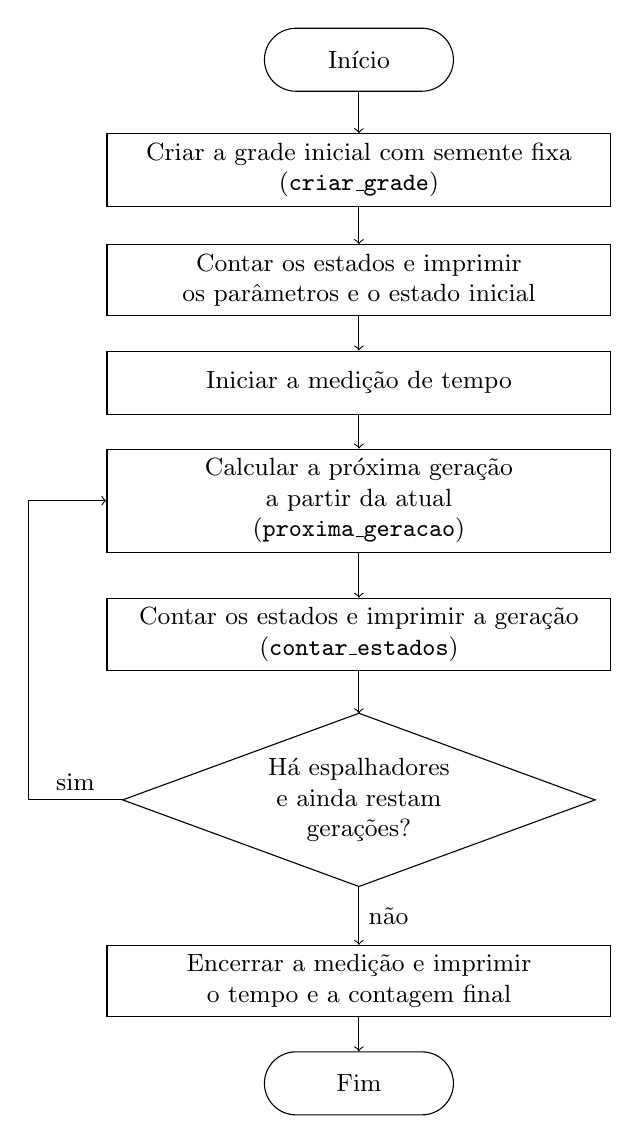
\begin{tikzpicture}[x=1cm, y=1cm, font=\small,
            etapa/.style={draw, align=center, minimum width=6.4cm, minimum height=0.8cm},
            extremo/.style={draw, rounded corners=0.4cm, minimum width=2.4cm, minimum height=0.8cm}]
        \node[extremo] (inicio) at (0, 0) {Início};
        \node[etapa] (criar) at (0, -1.4) {Criar a grade inicial com semente fixa\\(\texttt{criar\_grade})};
        \node[etapa] (inicial) at (0, -2.8) {Contar os estados e imprimir\\os parâmetros e o estado inicial};
        \node[etapa] (relogio) at (0, -4.1) {Iniciar a medição de tempo};
        \node[etapa] (proxima) at (0, -5.6) {Calcular a próxima geração\\a partir da atual\\(\texttt{proxima\_geracao})};
        \node[etapa] (contar) at (0, -7.3) {Contar os estados e imprimir a geração\\(\texttt{contar\_estados})};
        %% Losango desenhado com caminho próprio (sem biblioteca do TikZ)
        \draw (0, -8.3) -- (3.0, -9.4) -- (0, -10.5) -- (-3.0, -9.4) -- cycle;
        \node[align=center] at (0, -9.4) {Há espalhadores\\e ainda restam\\gerações?};
        \node[etapa] (final) at (0, -11.7) {Encerrar a medição e imprimir\\o tempo e a contagem final};
        \node[extremo] (fim) at (0, -13.0) {Fim};
        \draw[->] (inicio) -- (criar);
        \draw[->] (criar) -- (inicial);
        \draw[->] (inicial) -- (relogio);
        \draw[->] (relogio) -- (proxima);
        \draw[->] (proxima) -- (contar);
        \draw[->] (contar) -- (0, -8.3);
        \draw[->] (0, -10.5) -- node[right] {não} (final);
        \draw[->] (-3.0, -9.4) -- node[above] {sim} (-4.2, -9.4) |- (proxima.west);
        \draw[->] (final) -- (fim);
    \end{tikzpicture}
    \fonte{}
    \addcontentsline{loge}{figure}{\protect\numberline{\thefigure}Fluxograma da implementação sequencial}
\end{figure}

Primeiro, a grade inicial é criada e o estado inicial é impresso. Em seguida, cada iteração do laço calcula uma geração inteira e imprime a contagem dos estados. O laço termina quando não há mais espalhadores ou quando o número de gerações pedido é atingido; por fim, o programa imprime o tempo de execução e a distribuição final dos estados.

\subsection{Estrutura e funções}\label{sub:funcoes-sequencial}

A grade é uma lista de listas de inteiros, uma lista por linha, e os três estados são representados pelas constantes \texttt{IGNORANTE}~(0), \texttt{ESPALHADOR}~(1) e \texttt{INATIVO}~(2).

A função \texttt{criar\_grade} gera a população inicial. Ela inicializa o gerador pseudoaleatório do Python com \texttt{random.seed(semente)}, em que a semente vale 42 por padrão, preenche toda a grade com ignorantes e sorteia $\lfloor L \cdot C \cdot p \rfloor$ posições com \texttt{random.randint}, sendo $p$ o percentual inicial de espalhadores; cada posição sorteada torna-se espalhadora. O sorteio é feito com reposição: uma mesma célula pode ser sorteada mais de uma vez, e por isso o número real de espalhadores pode ser menor que o pedido. Na grade de $100 \times 100$ com 5\% de espalhadores, por exemplo, são feitos 500 sorteios, que resultam em 490 espalhadores; é por esse motivo que o programa imprime a quantidade de ``espalhadores reais''. Essa é a única parte aleatória do programa: como a semente é fixa, a mesma grade inicial é obtida em toda execução com os mesmos parâmetros.

A função \texttt{contar\_vizinhos\_espalhadores} recebe a grade e a posição $(i, j)$ de uma célula e conta quantos dos seus vizinhos na vizinhança de Moore são espalhadores. Para isso, percorre os deslocamentos $\Delta i, \Delta j \in \{-1, 0, 1\}$, descarta o par $(0, 0)$, que corresponde à própria célula, e só consulta a posição vizinha se ela estiver dentro da grade, isto é, se $0 \le i + \Delta i < L$ e $0 \le j + \Delta j < C$. É esse teste de limite que implementa as bordas fixas descritas na Seção~\ref{sec:automatos-celulares}: o vizinho que estaria fora da matriz simplesmente não é contado.

A função \texttt{proxima\_geracao} aplica as regras de transição a toda a grade. Ela cria a nova grade como uma cópia independente da atual (\texttt{deepcopy}) e percorre todas as células, linha a linha. Para cada célula ignorante, conta os vizinhos espalhadores e, se o total for maior ou igual ao limiar $\lambda$ (parâmetro \texttt{limiar\_convencimento}), marca a célula como espalhadora na nova grade; caso contrário, a célula mantém o valor copiado e continua ignorante. Cada espalhador passa a inativo, e cada inativo permanece inativo. A contagem de vizinhos é feita apenas para as células ignorantes, pois só elas mudam de estado por influência dos vizinhos. Durante toda a varredura, os estados são lidos somente da grade atual e escritos somente na nova grade; assim, nenhuma célula enxerga o estado já atualizado de um vizinho, o que implementa a atualização síncrona apresentada na Seção~\ref{sec:automatos-celulares}. Ao final, a nova grade é devolvida e passa a ser a grade atual.

A função \texttt{contar\_estados} percorre a grade inteira e devolve um dicionário com a quantidade de células em cada estado. Esses totais são usados tanto para imprimir o andamento da simulação quanto para decidir a parada. A função auxiliar \texttt{imprimir\_grade} mostra no terminal até $30 \times 30$ células da grade, com os símbolos ``.'', ``E'' e ``N'', e só é chamada quando a opção \texttt{mostrar\_grade} está ativada.

Por fim, a função \texttt{executar\_simulacao} coordena a execução descrita na Figura~\ref{fig:fluxograma-sequencial}. Seus parâmetros são o número de linhas e de colunas, o número máximo de gerações, o percentual inicial de espalhadores, o limiar de convencimento e a opção \texttt{mostrar\_grade}. Os valores padrão da função são uma grade de $100 \times 100$, 50~gerações, 2\% de espalhadores e limiar~2, mas o bloco principal do arquivo a chama com 5\% de espalhadores e limiar~3. Depois de criar a grade e imprimir os parâmetros e a contagem inicial, a função executa o laço de gerações; após cada geração, imprime uma linha com as quantidades de ignorantes, espalhadores e inativos e interrompe o laço antecipadamente se não houver mais espalhadores, já que, sem eles, nenhum ignorante pode ser convencido e a grade não muda mais. O tempo de execução é medido com \texttt{time.time()} imediatamente antes e depois do laço, de modo que o intervalo medido inclui o cálculo, a contagem e as impressões de cada geração. Ao final, são impressos esse tempo e a quantidade e o percentual de células em cada estado.

\subsection{Exemplo de execução}\label{sub:exemplo-sequencial}

Para ilustrar o funcionamento passo a passo, a Figura~\ref{fig:exemplo-sequencial} mostra a evolução de uma grade de $5 \times 5$ criada pela própria função \texttt{criar\_grade}, com semente~42 e 12\% de espalhadores (três sorteios, que resultaram em três espalhadores), e evoluída por \texttt{proxima\_geracao} com limiar $\lambda = 2$. As posições são indicadas por (linha, coluna), numeradas a partir de 0, como no código. Abaixo de cada grade aparecem as quantidades de ignorantes (I), espalhadores (E) e inativos (N), as mesmas que o programa imprime a cada geração.

\begin{figure}[!htb]
    \caption{Exemplo de evolução de uma grade de 5~$\times$~5 com limiar 2}
    \label{fig:exemplo-sequencial}
    \centering
    %% Gerado executando criar_grade(5, 5, 0.12) e proxima_geracao(grade, 2) do código fornecido.
    %% \painel{x}{y}{espalhadores}{inativos}{geração}{contagem}; posições em linha/coluna.
    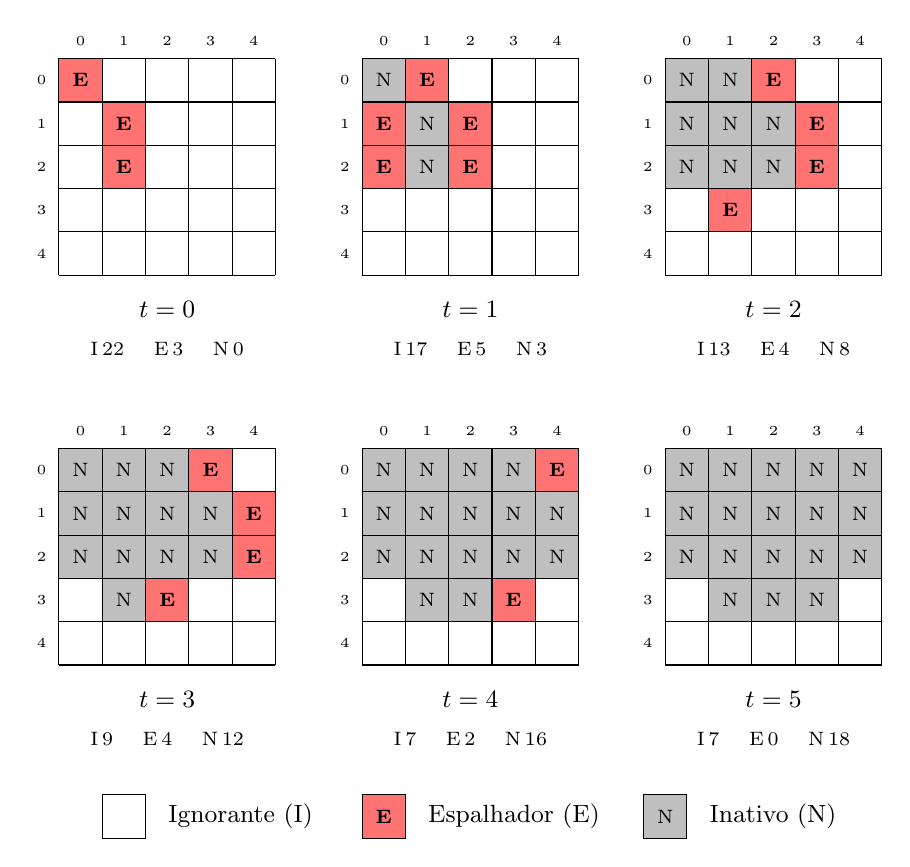
\begin{tikzpicture}[x=0.55cm, y=0.55cm]
        \newcommand*{\painel}[6]{%
            \begin{scope}[shift={(#1,#2)}]
                \foreach \i/\j in {#3} {\filldraw[fill=red!55] (\j,-\i) rectangle +(1,-1) node[midway] {\scriptsize\textbf{E}};}
                \foreach \i/\j in {#4} {\filldraw[fill=black!25] (\j,-\i) rectangle +(1,-1) node[midway] {\scriptsize N};}
                \foreach \k in {0,...,5} {\draw (\k,0) -- (\k,-5); \draw (0,-\k) -- (5,-\k);}
                \foreach \k in {0,...,4} {
                    \node[font=\tiny] at (\k+0.5, 0.4) {\k};
                    \node[font=\tiny] at (-0.4, -\k-0.5) {\k};
                }
                \node[font=\small] at (2.5,-5.8) {#5};
                \node[font=\scriptsize] at (2.5,-6.7) {#6};
            \end{scope}}
        \painel{0}{0}{0/0,1/1,2/1}{}{$t=0$}{I\,22 \quad E\,3 \quad N\,0}
        \painel{7}{0}{0/1,1/0,1/2,2/0,2/2}{0/0,1/1,2/1}{$t=1$}{I\,17 \quad E\,5 \quad N\,3}
        \painel{14}{0}{0/2,1/3,2/3,3/1}{0/0,0/1,1/0,1/1,1/2,2/0,2/1,2/2}{$t=2$}{I\,13 \quad E\,4 \quad N\,8}
        \painel{0}{-9}{0/3,1/4,2/4,3/2}{0/0,0/1,0/2,1/0,1/1,1/2,1/3,2/0,2/1,2/2,2/3,3/1}{$t=3$}{I\,9 \quad E\,4 \quad N\,12}
        \painel{7}{-9}{0/4,3/3}{0/0,0/1,0/2,0/3,1/0,1/1,1/2,1/3,1/4,2/0,2/1,2/2,2/3,2/4,3/1,3/2}{$t=4$}{I\,7 \quad E\,2 \quad N\,16}
        \painel{14}{-9}{}{0/0,0/1,0/2,0/3,0/4,1/0,1/1,1/2,1/3,1/4,2/0,2/1,2/2,2/3,2/4,3/1,3/2,3/3}{$t=5$}{I\,7 \quad E\,0 \quad N\,18}
        %% Legenda
        \draw (1,-17) rectangle +(1,-1);
        \node[anchor=west, font=\small] at (2.3,-17.5) {Ignorante (I)};
        \filldraw[fill=red!55] (7,-17) rectangle +(1,-1) node[midway] {\scriptsize\textbf{E}};
        \node[anchor=west, font=\small] at (8.3,-17.5) {Espalhador (E)};
        \filldraw[fill=black!25] (13.5,-17) rectangle +(1,-1) node[midway] {\scriptsize N};
        \node[anchor=west, font=\small] at (14.8,-17.5) {Inativo (N)};
    \end{tikzpicture}
    \fonte{}
    \addcontentsline{loge}{figure}{\protect\numberline{\thefigure}Exemplo de evolução de uma grade de 5~$\times$~5 com limiar 2}
\end{figure}

Na geração inicial ($t=0$), há espalhadores em (0,0), (1,1) e (2,1). A célula (1,0), na borda esquerda, tem apenas cinco vizinhos, mas três deles são espalhadores; as células (0,1), (1,2), (2,0) e (2,2) têm dois vizinhos espalhadores cada. Todas atingem o limiar e tornam-se espalhadoras em $t=1$. Já as células (0,2), (3,0), (3,1) e (3,2) têm apenas um vizinho espalhador e continuam ignorantes. Os três espalhadores iniciais tornam-se inativos: cada espalhador propaga a notícia durante uma única geração.

Em $t=1$, os cinco novos espalhadores formam uma frente em volta das células que se tornaram inativas. Convertem-se as células (0,2), (1,3) e (2,3), com dois vizinhos espalhadores cada, e (3,1), cujos vizinhos espalhadores são (2,0) e (2,2). A célula (2,1) também é vizinha de (3,1), mas, por estar inativa, não é contada: inativos não influenciam ninguém. A célula (3,0) tem novamente apenas um vizinho espalhador, (2,0), e continua ignorante.

Em $t=2$, a frente continua a avançar para a direita e para baixo. Tornam-se espalhadoras (0,3), (1,4) e (2,4), e também (3,2), cujos vizinhos espalhadores são (2,3) e (3,1). As demais células ignorantes têm no máximo um vizinho espalhador e não mudam; entre elas estão (3,0) e as células (4,0), (4,1) e (4,2) da última linha, vizinhas apenas de (3,1).

Em $t=3$, somente duas células atingem o limiar: (0,4), no canto superior direito, vizinha de (0,3) e (1,4), e (3,3), vizinha de (2,4) e (3,2). As outras células ignorantes, como (3,4) e as da última linha, têm no máximo um vizinho espalhador, e a frente começa a se desfazer.

Em $t=4$, os dois espalhadores restantes estão isolados: (0,4) só tem vizinhos inativos, e cada célula ignorante vizinha de (3,3), isto é, (3,4), (4,2), (4,3) e (4,4), tem apenas esse vizinho espalhador. Nenhuma célula é convertida, e em $t=5$ não há mais espalhadores. Nesse ponto, \texttt{executar\_simulacao} interrompe o laço, mesmo que o número de gerações pedido seja maior, e a grade termina com 7 ignorantes e 18 inativos: as células (3,0) e (3,4) e toda a última linha nunca tiveram dois vizinhos espalhadores na mesma geração.

O exemplo evidencia dois aspectos que determinam a dinâmica do modelo. Como cada espalhador atua por uma única geração, as influências recebidas em gerações diferentes não se acumulam: uma célula só é convertida se tiver ao menos $\lambda$ vizinhos espalhadores ao mesmo tempo. Por isso, quando a frente de propagação se estreita, por exemplo junto às bordas, onde há menos vizinhos, ela deixa de atingir o limiar, e a propagação se extingue antes de alcançar toda a população.

\subsection{Versão sequencial refatorada}\label{sub:sequencial-refatorada}

Além do código fornecido, foi desenvolvida uma versão sequencial refatorada (\texttt{sequencial/fakenews\_sequencial.py}), que usa o mesmo núcleo de cálculo das versões paralela e distribuída (\texttt{comum/modelo.py}). Ela mantém as regras de transição e a grade inicial, gerada pela própria função \texttt{criar\_grade} com a mesma semente, e muda apenas a representação dos dados: a grade passa a ser um vetor de bytes com uma linha de zeros acima e outra abaixo, e duas grades são alternadas entre as gerações, em vez de uma cópia com \texttt{deepcopy} a cada geração. Testes automatizados verificam que ela produz, geração a geração, as mesmas grades que o código original. Essa versão é a linha de base dos experimentos (Seção~\ref{cap:experimentos}), pois executa o mesmo cálculo das versões paralela e distribuída sem nenhum custo de comunicação ou de sincronização; seus detalhes são apresentados na Seção~\ref{cap:melhorias}. A seguir, analisa-se o custo computacional da implementação sequencial.

\section{Análise de custo}\label{sec:custo-sequencial}

Esta seção analisa o custo de tempo e de memória da implementação fornecida. Primeiro, o custo é estimado a partir do código; em seguida, a estimativa é comparada com medições, e discute-se como os parâmetros do modelo afetam a duração da simulação. As medições foram feitas com os \textit{scripts} da pasta \texttt{experimentos/} do repositório, sempre com a grade inicial de semente~42.

\subsection{Custo por geração}\label{sub:custo-geracao}

Em cada geração, \texttt{proxima\_geracao} copia a grade com \texttt{deepcopy} e visita uma vez cada uma das $L \cdot C$ células. O trabalho por célula depende do estado: uma célula ignorante chama \texttt{contar\_vizinhos\_espalhadores}, que percorre os nove deslocamentos da vizinhança, descarta o central e testa se cada vizinho está dentro da grade antes de consultá-lo, enquanto um espalhador ou um inativo exige apenas a comparação do estado e uma atribuição. Em seguida, \texttt{contar\_estados} percorre a grade inteira mais uma vez. Sendo $N_I$ o número de células ignorantes na geração, o tempo de uma geração pode ser escrito como
\begin{equation}\label{eq:custo-geracao}
    T_{\mathrm{ger}} \approx c_I \, N_I + c_O \, (L C - N_I) + (c_{\mathrm{cop}} + c_{\mathrm{cont}}) \, L C ,
\end{equation}
em que $c_I$ e $c_O$ são os custos de visitar uma célula ignorante e uma célula de outro estado, e $c_{\mathrm{cop}}$ e $c_{\mathrm{cont}}$ são os custos por célula da cópia e da contagem. Todos os termos são proporcionais ao tamanho da grade; logo, uma geração custa $\Theta(L \cdot C)$, e a simulação inteira custa $\Theta(G_{\mathrm{ef}} \cdot L \cdot C)$, em que $G_{\mathrm{ef}} \le G$ é o número de gerações efetivamente executadas, que pode ser menor que o pedido por causa da parada antecipada.

A memória também cresce com $L \cdot C$. A grade é uma lista de listas de inteiros; no CPython, cada posição de uma lista guarda uma referência de 8~bytes para um objeto inteiro, e os inteiros pequenos, como 0, 1 e 2, são objetos compartilhados. Por isso, a grade ocupa cerca de 8,9~bytes por célula, quase todos gastos com referências: 8,45~MiB para uma grade de $1000 \times 1000$, medidos com o módulo \texttt{tracemalloc}. Durante \texttt{proxima\_geracao}, a grade atual e a cópia existem ao mesmo tempo, e a memória ocupada dobra, chegando a cerca de 17~MiB nessa grade. Para comparação, a mesma grade guardada como vetor de bytes, como na versão refatorada, ocupa cerca de 1~byte por célula.

\subsection{Medições}\label{sub:custo-medicoes}

Para verificar a estimativa, a Tabela~\ref{tab:custo-escala} mostra o tempo do laço de gerações do código fornecido em três tamanhos de grade, com 20~gerações, 5\% de espalhadores e limiar~2, sem impressão no terminal. As medições foram feitas em um processador Intel Core i9-12900F, com Windows~11 e Python~3.11.7, e o valor apresentado é a mediana de três repetições.

\begin{table}[htb]
    \centering
    \caption{Tempo do laço de gerações do código fornecido conforme o tamanho da grade}
    \label{tab:custo-escala}
    \begin{tabular}{lrrrr}
        \toprule
        \textbf{Grade} & \textbf{Células} & \textbf{Tempo (s)} & \textbf{Por geração (s)} & \textbf{Por célula e geração ($\mu$s)} \\
        \midrule
        $500 \times 500$   & 250\,000     & 4,16  & 0,208 & 0,83 \\
        $1000 \times 1000$ & 1\,000\,000  & 16,46 & 0,823 & 0,82 \\
        $2000 \times 2000$ & 4\,000\,000  & 65,88 & 3,294 & 0,82 \\
        \bottomrule
    \end{tabular}
    \fonte{}
\end{table}

Quando o número de células é multiplicado por quatro, o tempo também é multiplicado por quatro, e o tempo por célula e por geração permanece em torno de 0,82~$\mu$s: o custo cresce linearmente com $L \cdot C$, como previsto. Esse valor corresponde a milhares de ciclos de relógio do processador por célula, o que reflete o custo de interpretar o código Python, em que cada acesso a uma lista, comparação ou chamada de função é executado pelo interpretador.

A Tabela~\ref{tab:custo-perfil} mostra como o tempo de uma geração se divide entre as etapas. Essa medição foi feita em outra máquina (Intel Core i7-13650HX, Windows~11, Python~3.12.10), na grade de $1000 \times 1000$ e com os mesmos parâmetros, e o valor apresentado é a mediana de cinco repetições, após uma execução de aquecimento descartada. Como o \texttt{deepcopy} ocorre dentro de \texttt{proxima\_geracao} e o código fornecido não foi alterado, a cópia foi medida à parte, sobre uma cópia da mesma grade, e o tempo da varredura foi obtido por diferença; os valores dessas duas linhas são, portanto, estimativas.

\begin{table}[htb]
    \centering
    \caption{Divisão do tempo de uma geração do código fornecido}
    \label{tab:custo-perfil}
    \begin{tabular}{lrr}
        \toprule
        \textbf{Etapa} & \textbf{Por geração (s)} & \textbf{Participação (\%)} \\
        \midrule
        Varredura das células                           & 0,638 & 74,6 \\
        Cópia da grade (\texttt{deepcopy})              & 0,179 & 21,0 \\
        Contagem dos estados (\texttt{contar\_estados}) & 0,038 & 4,4 \\
        \midrule
        Total                                          & 0,855 & 100,0 \\
        \bottomrule
    \end{tabular}
    \fonte{}
\end{table}

A varredura das células responde por cerca de três quartos do tempo, e a cópia, por cerca de um quinto. A cópia não contribui para o cálculo: ela pode ser evitada alternando duas grades entre as gerações, como faz a versão refatorada, cujo ganho é apresentado na Seção~\ref{cap:melhorias}.

O perfil também confirma que o custo depende do estado das células. Ao longo das 20~gerações, o número de ignorantes cai de cerca de 951~mil para 440~mil, e o tempo da varredura cai junto, com correlação de 0,999. Ajustando uma reta pelo método dos mínimos quadrados ao tempo da varredura em função do número de ignorantes, conforme a Equação~\ref{eq:custo-geracao}, obtêm-se $c_I \approx 1,02$~$\mu$s por célula ignorante e $c_O \approx 0,06$~$\mu$s por célula nos demais estados. Como $c_O$ vem do prolongamento da reta até $N_I = 0$, fora da faixa medida, seu valor é menos preciso que o de $c_I$; ainda assim, visitar um ignorante custa mais de dez vezes o que custa visitar uma célula de outro estado. Essa diferença faz com que regiões da grade com mais ignorantes demorem mais para ser calculadas, o que é a origem do desbalanceamento de carga discutido nas versões paralela e distribuída.

\subsection{Influência dos parâmetros}\label{sub:custo-parametros}

Como o custo total é $\Theta(G_{\mathrm{ef}} \cdot L \cdot C)$, o número de gerações efetivamente executadas também pesa, e ele depende fortemente do limiar e do percentual inicial de espalhadores. A Tabela~\ref{tab:custo-limiar} mostra, para a grade de $1000 \times 1000$, quantas gerações a simulação dura até não haver mais espalhadores e qual fração da população deixou de ser ignorante (alcance); em cada célula da tabela, o primeiro número é a quantidade de gerações e o valor entre parênteses é o alcance. Esses valores não dependem da máquina e foram obtidos com a versão refatorada, que produz as mesmas grades que o código fornecido.

\begin{table}[htb]
    \centering
    \caption{Gerações até a propagação terminar e alcance final, conforme o limiar e o percentual inicial de espalhadores}
    \label{tab:custo-limiar}
    \begin{tabular}{lrrrr}
        \toprule
        \textbf{Limiar} & \textbf{1\%} & \textbf{2\%} & \textbf{5\%} & \textbf{10\%} \\
        \midrule
        $\lambda = 1$ & 27 (100,0\%) & 15 (100,0\%) & 10 (100,0\%) & 7 (100,0\%) \\
        $\lambda = 2$ & 264 (14,3\%) & 163 (25,2\%) & 56 (57,9\%) & 29 (90,8\%) \\
        $\lambda = 3$ & 2 (1,0\%) & 3 (2,0\%) & 3 (5,4\%) & 4 (12,8\%) \\
        \bottomrule
    \end{tabular}
    \fonte{}
\end{table}

Com $\lambda = 1$, um único vizinho espalhador basta, e a notícia alcança toda a população em poucas gerações. Com $\lambda = 3$, é raro uma célula ter três vizinhos espalhadores ao mesmo tempo, e a propagação termina em até quatro gerações, alcançando pouco mais que os espalhadores iniciais. Com $\lambda = 2$, a simulação é a mais longa, chegando a 264~gerações com 1\% de espalhadores, e o alcance varia de 14\% a 91\% conforme o percentual inicial. Por isso, os parâmetros usados no bloco principal do código fornecido ($\lambda = 3$ e 5\%) encerram a simulação em três gerações e não servem para medir desempenho. Nos experimentos (Seção~\ref{cap:experimentos}), foram usados $\lambda = 2$ e 5\% de espalhadores com 20~gerações: como, nesse cenário, a propagação dura 56~gerações, todas as execuções completam as 20~gerações, e o trabalho medido é o mesmo em todas as versões.

\subsection{Potencial de paralelização}\label{sub:custo-paralelizacao}

A análise também indica o que pode ser paralelizado. O novo estado de cada célula depende apenas da geração anterior; portanto, as $L \cdot C$ atualizações de uma geração são independentes entre si e podem ser divididas entre vários trabalhadores, sem comunicação durante o cálculo. A contagem dos estados também pode ser feita por partes e somada ao final. A dependência existe apenas entre gerações: a geração $t+1$ só pode começar quando a geração $t$ estiver completa, e a decisão de parada exige a soma das contagens de toda a grade. Essas duas restrições definem os pontos de sincronização das versões paralela e distribuída, apresentadas nas seções~\ref{cap:paralela} e~\ref{cap:distribuida}.
%% Modelo computacional e versão sequencial
%%%% CAPÍTULO 4 - VERSÃO PARALELA

\chapter{Versão paralela}\label{cap:paralela}

\section{Estratégia de paralelização}

\todo{Linguagem e mecanismo escolhidos (\textit{threads} em Java ou \texttt{multiprocessing} em Python) e justificativa (GIL).}

\section{Divisão da matriz}

\todo{Decomposição por blocos de linhas; figura mostrando a divisão entre \textit{threads}; tratamento de divisão não exata.}

\section{Sincronização e consistência entre gerações}

\todo{Leitura da geração $t$ compartilhada (somente leitura), escrita exclusiva de cada \textit{thread} nas suas linhas da geração $t+1$; barreira ao fim de cada geração; redução da contagem de estados; por que não há condição de corrida.}

\section{Verificação de correção}

\todo{Comparação célula a célula com a versão sequencial.}
%% Versão paralela (threads/multiprocessing)
%%%% CAPÍTULO 5 - VERSÃO DISTRIBUÍDA

\chapter{Versão distribuída}\label{cap:distribuida}

\section{Arquitetura}

\todo{Coordenador e \textit{workers}; tecnologia (\textit{sockets} TCP ou RMI); diagrama da arquitetura.}

\section{Divisão da matriz entre processos}

\todo{Faixas de linhas por processo; linhas fantasmas (\textit{halo}) acima e abaixo.}

\section{Protocolo de comunicação}

\todo{Formato das mensagens; troca de fronteiras a cada geração; serialização; diagrama de sequência.}

\section{Sincronização e consistência das gerações}

\todo{Como se garante que todos estão na mesma geração; redução global do número de espalhadores para o critério de parada.}

\section{Verificação de correção}

\todo{Comparação célula a célula com a versão sequencial.}
%% Versão distribuída (sockets/RMI)
%%%% CAPÍTULO 6 - MELHORIAS E EXTENSÕES
%% Cada melhoria vale até 0,5 ponto (máximo 3,0). Para cada uma:
%% motivação, descrição técnica, referência e resultado/evidência.

\chapter{Melhorias e extensões}\label{cap:melhorias}

Este capítulo descreve as melhorias propostas sobre o modelo e a implementação originais. Para cada uma são apresentadas a motivação, a solução adotada, a fundamentação e o impacto observado.

\section{Melhoria 1: \todo{nome}}

\textbf{Motivação.} \todo{}

\textbf{Implementação.} \todo{}

\textbf{Fundamentação.} \todo{}

\textbf{Resultado.} \todo{}

%% Copiar o bloco acima para cada melhoria adicional.
%% Melhorias e extensões
%%%% CAPÍTULO 7 - EXPERIMENTOS E RESULTADOS

\chapter{Experimentos e resultados}\label{cap:experimentos}

\section{Configuração experimental}

Os experimentos de desempenho foram executados em duas máquinas, descritas na Tabela~\ref{tab:ambiente}: um computador de mesa com Windows (Máquina~A), em que foi feita a bateria principal, e um \textit{notebook} com Linux (Máquina~B), em que a mesma bateria foi repetida para comparação. Os resultados de cada máquina são apresentados separadamente: tempos de máquinas ou sistemas operacionais diferentes não são combinados num mesmo cálculo de \textit{speedup}. A análise de custo da Seção~\ref{sub:custo-medicoes} usou ainda uma terceira máquina, indicada naquela seção. Em todas as medições, a versão distribuída foi executada em uma única máquina, com os processos comunicando-se pela interface local (\textit{localhost}).

\begin{table}[htb]
    \centering
    \caption{Ambiente de execução dos experimentos}
    \label{tab:ambiente}
    \begin{tabular}{lp{5cm}p{5cm}}
        \toprule
        \textbf{Item} & \textbf{Máquina A (Windows)} & \textbf{Máquina B (Linux)} \\
        \midrule
        Processador & Intel Core i9-12900F & Intel Core i5-1240P \\
        Núcleos físicos / lógicos & 16 (8 de desempenho e 8 de eficiência) / 24 & 12 (4 de desempenho e 8 de eficiência) / 16 \\
        Memória RAM & 31,8~GB & 15,3~GB \\
        Sistema operacional & Windows~11 & Fedora Linux~44 (\textit{kernel} 7.3.3) \\
        Linguagem e versão & Python~3.11.7 (CPython) & Python~3.12.16 (CPython) \\
        Ambiente de execução & computador de mesa ligado na tomada, demais programas fechados & \textit{notebook} ligado na tomada, política de frequência do processador em \texttt{performance} \\
        \bottomrule
    \end{tabular}
    \fonte{}%% vazio = "Fonte: Autoria própria (ano)"
\end{table}

\section{Cenários avaliados}

As medições foram feitas por scripts do repositório (\texttt{experimentos/medir.py} e \texttt{experimentos/analisar.py}), e nenhuma tabela foi preenchida à mão. A bateria principal usou grades quadradas de $1000 \times 1000$ e $2000 \times 2000$ (e de $500 \times 500$ apenas para as versões sequenciais), com 20~gerações, 5\% de espalhadores iniciais e limiar~2, e mediu seis versões: o código original, a sequencial refatorada, a paralela com processos, a paralela com \textit{threads} e a distribuída em \textit{localhost}, com e sem a compactação das fronteiras em \textit{bits}. As versões paralelas e distribuídas foram executadas com 1, 2, 4, 8, 16 e 24 unidades de processamento na Máquina~A e com 1, 2, 4, 8, 12 e 16 na Máquina~B. O limiar~3 do código original não foi usado porque, com ele, a propagação termina em cerca de três gerações (Tabela~\ref{tab:custo-limiar}), o que não deixa tempo para medir.

Cada configuração foi executada uma vez para aquecimento, com o resultado descartado, e depois repetida ao menos cinco vezes; na Máquina~A, o código original, por ser o mais lento, e a grade de $500 \times 500$ foram repetidos três vezes. Reporta-se a mediana do tempo do laço de gerações, menos sensível que a média a execuções perturbadas pelo sistema operacional, acompanhada do desvio padrão, e o \textit{speedup} é calculado contra a sequencial refatorada da mesma máquina, cujo tempo absoluto é informado junto, como recomendam \citeonline{HoeflerBelli2015}. O tempo do laço começa depois que a grade inicial foi gerada e, nas versões paralela e distribuída, depois que os processos e as conexões foram criados; o tempo total, que inclui essa preparação, é registrado à parte. Toda execução grava o resumo SHA-256 da grade final, e a análise confere que ele é igual em todas as versões, de modo que cada bateria também funciona como um teste de equivalência em escala. O perfil de tempo por \textit{worker} foi coletado em execuções separadas, com a melhoria de estatísticas ligada (Seção~\ref{sec:melhoria-estatisticas}).

\todo{Acrescentar os cenários das baterias finais: variação do percentual de espalhadores, do limiar e do número de gerações, e a execução entre três máquinas.}

\section{Resultados da versão paralela}

\todo{Tabela de tempos, gráficos de \textit{speedup} e eficiência.}

\section{Resultados da versão distribuída}

\todo{Tabela de tempos, gráficos de \textit{speedup} e eficiência; tempo de comunicação vs. cômputo.}

\section{Comparação entre as duas máquinas}\label{sec:comparacao-maquinas}

Para verificar se o comportamento observado depende da máquina e do sistema operacional, a bateria da grade de $1000 \times 1000$ foi repetida na Máquina~B, com Linux, usando os mesmos parâmetros: 20~gerações, 5\% de espalhadores, limiar~2, uma execução de aquecimento descartada e cinco repetições, das quais se reporta a mediana do tempo do laço de gerações. A Tabela~\ref{tab:comparacao-maquinas} mostra os tempos e o \textit{speedup} de cada máquina, sempre calculado contra a sequencial refatorada da própria máquina. Na Máquina~A, o código fornecido foi medido com três repetições, por ser o mais lento.

\begin{table}[htb]
    \centering
    \caption{Tempo do laço e \textit{speedup} na grade de $1000 \times 1000$ em cada máquina}
    \label{tab:comparacao-maquinas}
    \begin{tabular}{lrrrrr}
        \toprule
        & & \multicolumn{2}{c}{\textbf{Máquina A (Windows)}} & \multicolumn{2}{c}{\textbf{Máquina B (Linux)}} \\
        \textbf{Versão} & \textbf{\textit{Workers}} & \textbf{Tempo (s)} & \textbf{\textit{Speedup}} & \textbf{Tempo (s)} & \textbf{\textit{Speedup}} \\
        \midrule
        Sequencial (fornecida)  & 1  & 16,46 & 0,30 & 14,40 & 0,31 \\
        Sequencial (refatorada) & 1  & 4,94  & 1,00 & 4,50  & 1,00 \\
        \midrule
        Paralela (processos)    & 1  & 4,97  & 0,99 & 4,76  & 0,95 \\
                                & 2  & 2,22  & 2,23 & 2,54  & 1,77 \\
                                & 4  & 1,16  & 4,25 & 1,57  & 2,86 \\
                                & 8  & 0,71  & 6,94 & 1,22  & 3,68 \\
                                & 16 & 0,51  & 9,61 & 1,02  & 4,42 \\
        Paralela (\textit{threads}) & 8 & 5,30 & 0,93 & 4,85 & 0,93 \\
        \midrule
        Distribuída (\textit{localhost}) & 1  & 4,97 & 0,99 & 4,82 & 0,93 \\
                                & 2  & 2,17  & 2,27 & 2,64  & 1,70 \\
                                & 4  & 1,19  & 4,16 & 1,58  & 2,85 \\
                                & 8  & 0,73  & 6,74 & 1,25  & 3,59 \\
                                & 16 & 0,53  & 9,30 & 1,01  & 4,45 \\
        \bottomrule
    \end{tabular}
    \fonte{}
\end{table}

Nas duas máquinas, todas as execuções produziram a mesma grade final, conferida pelo resumo SHA-256 da grade: na Máquina~B foram 130~medições, todas idênticas à sequencial. A suíte de testes automatizados do projeto também passou nos dois sistemas operacionais, sem alteração no código: na Máquina~B, os 76~testes da versão final passaram com Python~3.12.16 e 3.14.10; na Máquina~A, a suíte passou com Python~3.11.7 e 3.12.10, quando ainda tinha 72~testes. O ganho da sequencial refatorada sobre o código fornecido foi semelhante nas duas máquinas (3,3$\times$ na Máquina~A e 3,2$\times$ na Máquina~B), e as \textit{threads} não trouxeram ganho em nenhuma delas (\textit{speedup} entre 0,88 e 0,99 na Máquina~B, para 1 a 16 \textit{threads}), pelo efeito do \ac{GIL}.

A escalabilidade, por outro lado, foi bem menor na Máquina~B. Com quatro \textit{workers}, a eficiência já caiu para 0,71, contra 1,06 na Máquina~A, e o \textit{speedup} parou de crescer entre 12 e 16 \textit{workers}, em torno de 4,4 a 4,6, enquanto a Máquina~A chegou a 9,6 com 16 processos. O comportamento é coerente com a configuração da Máquina~B, que tem apenas quatro núcleos de desempenho, e com o limite de potência de um processador de \textit{notebook}: quando parte das faixas fica nos núcleos de eficiência, mais lentos, a faixa mais lenta passa a determinar o tempo de cada geração, pois todos os \textit{workers} se sincronizam ao fim dela. A medição não registrou em qual núcleo cada \textit{worker} executou, então essa explicação não foi confirmada diretamente. A diferença no tempo de um único núcleo (o código fornecido levou 14,40~s na Máquina~B e 16,46~s na Máquina~A) não pode ser atribuída só ao sistema operacional, pois as versões do Python também são diferentes (3.12 e 3.11).

\section{Análise}

\subsection{Gargalos}
\todo{}

\subsection{Sincronização}
\todo{}

\subsection{Custo de comunicação}
\todo{}

\subsection{Limitações observadas}
\todo{}
%% Configuração experimental e resultados
%%%% CAPÍTULO 8 - CONCLUSÕES

\chapter{Conclusões}\label{cap:conclusoes}

\todo{Síntese dos resultados: o que foi obtido em \textit{speedup}/eficiência e por quê.}

\section{Dificuldades encontradas}

\todo{}

\section{Trabalhos futuros}

\todo{}

\section{Contribuição individual dos integrantes}

\begin{table}[htb]
    \centering
    \caption{Contribuição de cada integrante}
    \label{tab:contribuicoes}
    \begin{tabular}{lp{10cm}}
        \toprule
        \textbf{Integrante} & \textbf{Contribuição} \\
        \midrule
        \todo{Nome} & \todo{} \\
        \todo{Nome} & \todo{} \\
        \todo{Nome} & \todo{} \\
        \bottomrule
    \end{tabular}
    \fonte{}%% vazio = "Fonte: Autoria própria (ano)"
\end{table}
%% Conclusões, dificuldades e contribuições

%% ===== Elementos pós-textuais =====
\postextual

%% Referências: arquivos .bib sem a extensão, separados por vírgula
\arquivosdereferencias{main}

%% Títulos dos apêndices: negrito, tamanho normal, letra no lugar do número
\renewcommand{\ABNTEXchapterfont}{\bfseries}
\renewcommand{\ABNTEXchapterfontsize}{\normalsize}
\renewcommand{\thechapter}{\Alph{chapter}}
\renewcommand{\chaptername}{Apêndice}

%% Apêndices (produzidos pelos autores)
\begin{arquivosdeapendices}
  %%%% APÊNDICE A - INSTRUÇÕES DE EXECUÇÃO E USO DE FERRAMENTAS

\chapter{Instruções de execução}\label{apendice:execucao}

\todo{Requisitos (versão do Python/Java), como executar as versões sequencial, paralela e distribuída, parâmetros de linha de comando e como reproduzir os experimentos.}

\section{Uso de inteligência artificial generativa e código externo}

Conforme exigido no enunciado do trabalho, registra-se aqui toda utilização de IA generativa, código externo e bibliotecas adicionais.

\todo{Listar ferramenta, versão, finalidade e partes do trabalho em que foi usada.}
%% Instruções de execução e uso de IA
\end{arquivosdeapendices}

%% Anexos (documentos de terceiros), se houver:
%\begin{arquivosdeanexos}
%  %%%% ANEXO A
%%
%% Texto ou documento não elaborado pelo autor, que serve de fundamentação, comprovação e ilustração.

%% Título e rótulo de anexo (rótulos não devem conter caracteres especiais, acentuados ou cedilha)
\anexos
  \cleardoublepage
    \thispagestyle{empty}
    \refstepcounter{chapter} % incrementa o contador
    %\chapter*{Apêndice~\thechapter\\[1ex]Questionário de pesquisa}   
    \vspace*{\fill}
    \begin{center}
        {\bfseries ANEXO~\thechapter{ -- }Lei N\texorpdfstring{.\textsuperscript{o}}{o.} 9.610, de 19 de Fevereiro de 1998}
    \end{center}
    \vspace*{\fill}
    \addcontentsline{toc}{chapter}{ANEXO~\thechapter{ -- }Lei N\texorpdfstring{.\textsuperscript{o}}{o.} 9.610, de 19 de Fevereiro de 1998}

%\chapter{Lei N\texorpdfstring{.\textsuperscript{o}}{o.} 9.610, de 19 de Fevereiro de 1998}\label{cap:anexoa}


\newpage
\centerline{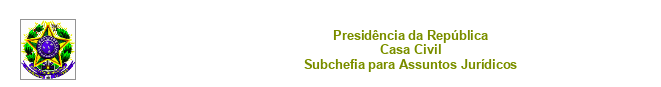
\includegraphics[width=\textwidth]{./PosTexto/Ilustracoes/top.png}}%% Imagem (Dimensões e localização)

\begin{center}
\textbf{LEI Nº 9.610, DE 19 DE FEVEREIRO DE 1998\footnote{Disponível em:\url{http://www.planalto.gov.br/ccivil_03/leis/l9610.htm.}}.}
\end{center}

\hspace{7cm}\parbox{8cm}{\scriptsize{\textcolor{red}{Altera, atualiza e consolida a legislação sobre direitos autorais e dá outras providências.}}}
\vspace{0.3cm}

\textbf{O PRESIDENTE DA REPÚBLICA} Faço saber que o Congresso Nacional decreta e eu sanciono a seguinte Lei:

\begin{center}
Título I - Disposições Preliminares
\end{center}

\scriptsize{
Art. 1º Esta Lei regula os direitos autorais, entendendo-se sob esta denominação os direitos de autor e os que lhes são conexos. 

Art. 2º Os estrangeiros domiciliados no exterior gozarão da proteção assegurada nos acordos, convenções e tratados em vigor no Brasil.

Parágrafo único. Aplica-se o disposto nesta Lei aos nacionais ou pessoas domiciliadas em país que assegure aos brasileiros ou pessoas domiciliadas no Brasil a reciprocidade na proteção aos direitos autorais ou equivalentes.

Art. 3º Os direitos autorais reputam-se, para os efeitos legais, bens móveis.

Art. 4º Interpretam-se restritivamente os negócios jurídicos sobre os direitos autorais.

Art. 5º Para os efeitos desta Lei, considera-se:

I - publicação - o oferecimento de obra literária, artística ou científica ao conhecimento do público, com o consentimento do autor, ou de qualquer outro titular de direito de autor, por qualquer forma ou processo;

II - transmissão ou emissão - a difusão de sons ou de sons e imagens, por meio de ondas radioelétricas; sinais de satélite; fio, cabo ou outro condutor; meios óticos ou qualquer outro processo eletromagnético; 

III - retransmissão - a emissão simultânea da transmissão de uma empresa por outra;

IV - distribuição - a colocação à disposição do público do original ou cópia de obras literárias, artísticas ou científicas, interpretações ou execuções fixadas e fonogramas, mediante a venda, locação ou qualquer outra forma de transferência de propriedade ou posse;

V - comunicação ao público - ato mediante o qual a obra é colocada ao alcance do público, por qualquer meio ou procedimento e que não consista na distribuição de exemplares;

VI - reprodução - a cópia de um ou vários exemplares de uma obra literária, artística ou científica ou de um fonograma, de qualquer forma tangível, incluindo qualquer armazenamento permanente ou temporário por meios eletrônicos ou qualquer outro meio de fixação que venha a ser desenvolvido;

VII - contrafação - a reprodução não autorizada;

VIII - obra: 

a) em co-autoria - quando é criada em comum, por dois ou mais autores;

b) anônima - quando não se indica o nome do autor, por sua vontade ou por ser desconhecido;

c) pseudônima - quando o autor se oculta sob nome suposto;

d) inédita - a que não haja sido objeto de publicação;

e) póstuma - a que se publique após a morte do autor;

f) originária - a criação primígena;

g) derivada - a que, constituindo criação intelectual nova, resulta da transformação de obra originária;

h) coletiva - a criada por iniciativa, organização e responsabilidade de uma pessoa física ou jurídica, que a publica sob seu nome ou marca e que é constituída pela participação de diferentes autores, cujas contribuições se fundem numa criação autônoma;

i) audiovisual - a que resulta da fixação de imagens com ou sem som, que tenha a finalidade de criar, por meio de sua reprodução, a impressão de movimento, independentemente dos processos de sua captação, do suporte usado inicial ou posteriormente para fixá-lo, bem como dos meios utilizados para sua veiculação;

IX - fonograma - toda fixação de sons de uma execução ou interpretação ou de outros sons, ou de uma representação de sons que não seja uma fixação incluída em uma obra audiovisual;

X - editor - a pessoa física ou jurídica à qual se atribui o direito exclusivo de reprodução da obra e o dever de divulgá-la, nos limites previstos no contrato de edição; 

XI - produtor - a pessoa física ou jurídica que toma a iniciativa e tem a responsabilidade econômica da primeira fixação do fonograma ou da obra audiovisual, qualquer que seja a natureza do suporte utilizado;

XII - radiodifusão - a transmissão sem fio, inclusive por satélites, de sons ou imagens e sons ou das representações desses, para recepção ao público e a transmissão de sinais codificados, quando os meios de decodificação sejam oferecidos ao público pelo organismo de radiodifusão ou com seu consentimento;

XIII - artistas intérpretes ou executantes - todos os atores, cantores, músicos, bailarinos ou outras pessoas que representem um papel, cantem, recitem, declamem, interpretem ou executem em qualquer forma obras literárias ou artísticas ou expressões do folclore.

Art. 6º Não serão de domínio da União, dos Estados, do Distrito Federal ou dos Municípios as obras por eles simplesmente subvencionadas.
}


%\end{arquivosdeanexos}

\end{document}
